\documentclass[a5paper]{scrreprt}
\usepackage{hyperref}
\usepackage{enumitem}
\usepackage{amsfonts}
\usepackage{float}
\usepackage{wrapfig}
\usepackage{graphicx}
\graphicspath{ {images/} }

\setlength\intextsep{0pt}

\begin{document}

\title{Software Requirements Specification for Smart History}
\subtitle{Chrome Browser Extension}
\date{\today}
\author{X-Space}

\maketitle

\tableofcontents

\chapter{Introduction}

\section{Purpose}

The purpose of this document is to describe the Smart History, an extension on 
chrome browser. This document contains the functional behavioral of the project 
and it also contains the nonfunctional requirements for users and developers to 
use or start working on this project.

\section{Project Scope}

Smart History is based on the history records of chrome. It provides a 
user-friendly graphic interface and enables users to have a better experience when 
searching history.

Users can use Smart History to filter the history, view the statistics about their
surfing pattern on the internet. Moreover, Smart History also automatically 
organizes the history and group related webs and even allow user to take notes or 
screenshots when working on webs.

\section{References}

\begin{itemize}
	\item \href{https://developer.chrome.com/extensions}{Chrome developer guide book}
	\item \href{http://www.w3schools.com/}{w3schools web developer site}
\end{itemize}


\chapter{Overall Description}

\section{Product Perspective}

Smart History can be a good replacement of origin chrome history page. Beside basic 
listing, searching and erasing functions, Smart History provides more useful functions 
with fancier GUI.

\section{Product Functions}

\begin{itemize}[label={\checkmark}]
	\item List all history.
	\item View history in specific time interval.
	\item View most visited history.
	\item View history with or without particular patterns.
	\item Erase any history in any views above.
	\item Search history by key words.
	\item Group related history records.
	\item Take and store screenshots.
	\item Add tags to page.
\end{itemize}

\section{User Classes and Characteristics}

Smart History aim to all chrome browser users. And it is especially helpful 
for those users working on their personal laptops or work stations who have needs 
to frequently review the information they viewed on the Internet.

\section{Operating Environment}

Smart History is developed and tested on chrome browser. But it use the basic
elements in web design like HTML, CSS, JSON and Javascript. So it can be applied
on other browsers with minor adaptation if the browser offers the history API.

\section{Design and Implementation Constraints}

Saving screen-shot may ask permit to access local storage. All other functions 
only require access to chrome history.

\section{Assumptions and Dependencies}

Smart History use chrome history as one and only data source, so it will not
list any browse records in incognito mode. No Internet connection is needed 
for all Smart History features, so there is no need to worry about privacy leak.


\chapter{External Interface Requirements}

\section{User Interfaces}

Smart History has three components: \textbf{Icon}, \textbf{Popup Window} and 
\textbf{History Page}.

\subsection{Icon}

Smart History will create a Icon pinned to the toolbar. (see Figure 3.1) Users 
can hide it any time in \href{chrome://extensions}{chrome extensions setting page}, 
or right click on the icon and select the hide option.

\begin{figure}[h]
	\centering
	\vspace{10pt}
	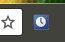
\includegraphics{spec_icon}
	\vspace{-10pt}
	\caption{Icon demo}
\end{figure}

\subsection{Popup Window}

{

Popup Window will show up when user click the Icon. It will list 
several latest history records and has some common features available, like 
screenshot, note, tag and search. (see Figure 3.2)

The title button is placed on the top left of the Popup Window. User can go to the 
History Page by clicking the title.

\begin{wrapfigure}{r}{0.55\textwidth}
	\centering
	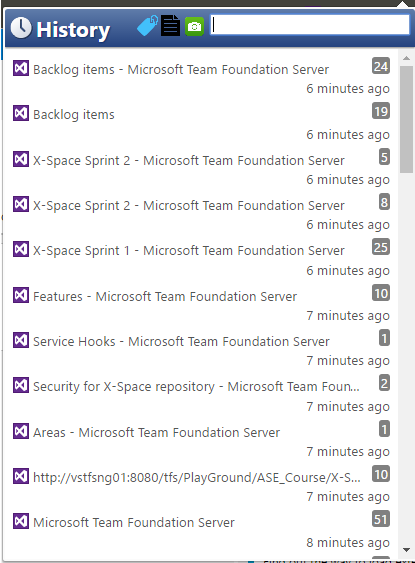
\includegraphics[width=0.55\textwidth]{spec_popup_window}
	\vspace{-22pt}
	\caption{Popup Window demo}
\end{wrapfigure}

On the right side of the title are three icons representing tag, note and 
screenshot. Users can click the icon to use corresponding features.

On the top right is a text box. User can type in key words and press enter to 
search related history records.

Below list the latest opened pages. Each history record is attached with last visit 
time and hit rate. User can access the websites by clicking on the list items.

}

\subsection{History Page}

{

\begin{wrapfigure}{l}{0.52\textwidth}
	\centering
	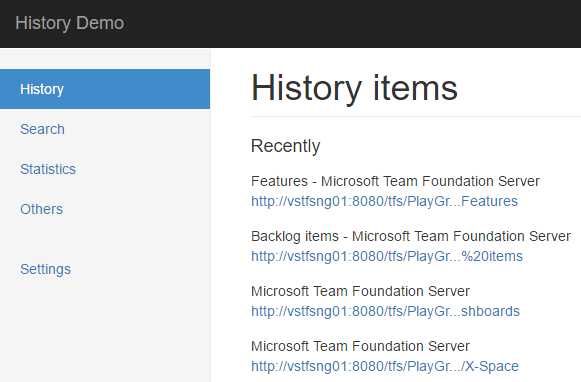
\includegraphics[width=0.52\textwidth]{spec_history_page}
	\vspace{-20pt}
	\caption{History Page demo}
\end{wrapfigure}

History page consists of two main components: Option tabs and Result window.

User can switch from different features on the left side panel. The result will 
be presented on the right side window.

}

In the Search tab, there are some fine-grained option to filter the result by 
date, hit rate, domain, tags, regular expressions, etc.

In the Statistics tab, users can learn their behavior from several charts, like 
most visited webs/domains, time distribution among domains, etc.

New features will be added into the Other tab base on feedback from users.

Users can set some rules to automatically filter some untitled pages or other 
pages they do not want to record. Smart History will provide several default rules, 
user can also set their own rules using regular expression.

Besides, there will be a mini box in the bottom left corner playing the animation 
of top hit pages. The pages will be show as their titles and keep rotating. So 
users can access these pages by clicking on them.


\section{Software Interfaces}

Smart History will use basic HTML elements and Javascript functions to 
demonstrate pages. The chrome history API will be the only data source. No 
other system requirements if chrome browser runs well.

In default, Smart History will override the chrome history as self-defined 
History Page. User can block the option in the Setting tab in History Page.


\chapter{System Features}

\section{List all history}

Smart History will automatically list dozens of latest history records in the 
Popup Window and all history records in the History Page.

The history record will contain the title, url, hit rate, last visited time 
and the logo of each website.

Each listed item will contain a hyperlink point to corresponding web, which 
can be trigger when users click on it.

\paragraph{Priority} This is the most basic feature of Smart History and have the 
highest priority.

\section{Filter history}

Users can use default and self-defined rules to filter the history records. The 
rules are written as regular expressions or set as a time scale. Once the rules 
are applied, the listed history records will not include those match the rules.

User can also define temporary rules in search options. These temporary rules 
contains four types: time scale, hit rate, domain pattern and key words. They 
can be applied separately or in any combination.

\paragraph{Priority} Filtering function will be used most frequently by users, 
so it also has the highest priority.

\section{Erase history}

Users can select and erase any number of history in any record list.

Smart History also support delete history records by self-defined rules. Users can 
simply select some rules and delete all matched records. Users can also do the 
search first and then select records and delete them.

\paragraph{Priority} Erase history is a basic function of origin chrome history 
page. Since Smart History override that page, it also share the same priority 
with filtering and listing functions.

\section{Group history}

Smart History will group history according to domain names and transition types.

View history as a group can help users better acquire related information. Also, 
some pages are actually different part of one single theme. It is redundant and 
messy to list all of them.

\paragraph{Priority} This feature will be a highlight of Smart History and distinct 
it from other similar extensions. So it has the priority right below the three core 
functions.

\section{Take notes}

Users may want to record some information of one page. Smart History provide users 
a fast way to add tag, write down some notes and take a screenshot on the web. The 
tags can also be used in key word search feature.

\paragraph{Priority} Users can use other excellent extensions to take notes. However, 
Smart History combined it with history records for better organizing. So it has the 
third priority.


\chapter{Other Nonfunctional Requirements}

\section{Performance Requirements}

\begin{itemize}[label=\checkmark]
	\item The search result should be given with a very short latency.
	\item Graphic User Interface should be user-friendly, most filter rules 
		should be implemented by button and checkbox.
\end{itemize}

\section{Security Requirements}

\begin{itemize}[label=\checkmark]
	\item Smart History MUST not sent history records to ANY entity.
\end{itemize}

\section{Software Quality Attributes}

\begin{itemize}[label=\checkmark]
	\item Smart History should define the rules of regular expression it can 
		process. These rules should be explicit and succinct.
\end{itemize}

\end{document}